\documentclass[conference,final]{IEEEtran}

\usepackage{graphicx}
\usepackage{epsfig}
\usepackage{subfigure}
\usepackage[hypertex]{hyperref}
\usepackage{subfigure}  
\usepackage{color}
% \usepackage{draftcopy}

\usepackage[small,it]{caption}

\usepackage{multirow}
\usepackage{ifpdf}

\long\def\comment#1{{ \bf \textcolor{magenta}{\bf #1}}}
\long\def\ccomment#1{{ \bf \textcolor{blue}{\bf #1 (SJ)}}}
\newcommand{\F}[1]{\B{\textcolor{red}{FIXME: #1}}}
\newcommand{\C}{\comment}
\newcommand{\CC}{\ccomment}
\newcommand{\fix}[1]{\textcolor{red}{\bf #1}}

\newcommand{\jha}[0]{}
\newcommand{\hartmut}[0]{}
\newcommand{\yaakoub}[0]{}
\newcommand{\ole}[0]{}

\newcommand{\fixme}[1]{ { \bf{ ***FIXME: #1 }} }
\newcommand{\jhanote}[1]{ {\textcolor{red} { ***Jha: #1 }}}
%\newcommand{\jhanote}[0]{}
\newcommand{\jitter}[1]{{$\sigma(\alpha)$}}

\newif\ifpdf
\ifx\pdfoutput\undefined
  \pdffalse
\else
  \ifnum\pdfoutput=1
    \pdftrue
  \else
    \pdffalse
  \fi
\fi

\ifpdf
\DeclareGraphicsExtensions{.pdf, .jpg}
\else
\DeclareGraphicsExtensions{.eps}
\fi

\begin{document}

\title{\large Developing Adaptive Scientific Applications with Hard to
  Predict Runtime Resource Requirements}

\author{\authorblockN{Shantenu Jha\authorrefmark{1}\authorrefmark{2},
    Yaakoub El Khamra\authorrefmark{1}, Hartmut
    Kaiser~\authorrefmark{1}, Andre Merzky{1}, Ole
    Weidner\authorrefmark{1}} \authorblockA{\authorrefmark{1} Center
    for Computation and Technology, Louisiana State University, Baton
    Rouge, 70803} \authorblockA{\authorrefmark{2} Department of
    Computer Science, Louisiana State University, Baton Rouge, 70803}
}
\maketitle

\begin{abstract}
  There exist a large class of applications that have irregular
  execution characteristics and highly variable resource requirements
  which are very difficult to predict in advance.  Not only is the
  development of such applications difficult, but the effective
  deployment of such application remains a challenge.  For example, as
  a consequence of irregular execution characteristics dynamic
  resource requirements are difficult to predict a priori thus
  rendering static resource mapping techniques such as workflows
  ineffective.  This paper discusses the design and development of an
  application for simulating oil reservoir which has varying resource
  requirements and execution characteristics. Even for relatively
  small input problem sizes at each stage, up to several hundred models
  are generated which require from one to sixteen processors; the
  distribution of the number of jobs and the run time-to-completion
  for a given processor count varies by up to an order of magnitude.
  Such hard to predict run-time characteristics render static,
  data-flow independent scheduling techniques not usable. We
  demonstrate how the use of appropriate programming abstractions like
  SAGA and Cactus enable the effective development of applications
  with non-trivial requirements, e.g., run-time resource selection
  based upon the application specific characteristics.  As proof of
  concept we deploy our application on the TeraGrid and show the
  effective utilization of several heterogeneous resources.
\end{abstract}

\begin{keywords}
  eScience Application, Middleware Inter-operation, Distributed
  Infrastructure Deployment, Distributed Application Programming,
  Cactus, Performance, SAGA, Lightpaths
\end{keywords}

\section{Introduction}\C{Jha}

There exist several well known examples of distributed applications
which in turn have multiple 'embarassingly' distributed jobs (or
sub-applications) that are either typically uncoupled or the coupling
is between the master-client application.  Things get significantly
more complicated when there is a horizontal coupling between the
distributed jobs say for example a global exchange or synchronization
point.  Most applications and support-tools for distributed
applications assume that the individual ``jobs'' during the course of
their run life-time will display a well-defined, static execution
characterisitcs.

However there are class of applications for which the individual job
run time characterisitcs are inherently difficult to predict and plan
for. Not suprisingly such applications are harder to develop and
deploy, but also they have traditionally not received the same level
of infrastructural support for the development.  

There exist a large set of scientific applications that fall into this
class. In addition to Parallel Kalman Filters -- a specific example of
which is the ``Black Oil'' (discussed in detailed in section 3) -- an
important application in petroleum engineering, there are ``first
principles'' Grid applications, such as GridSAT~\cite{gridsat03} and
applications which based upon resource aware ``learning''
algorithms~\cite{ majority_voting}, which need to explicitly marshal
distributed resources. For these applications the resource requirement
is often dynamic and unpredictable; interestingly, the resource
requirements and utilization might possibly be dependent upon both the
execution trajectory and underlying infrastructure. It is difficult to
define a scheduling strategy that will be effective throughtout the
exection of a complete application.

Grids are inherently dynamic; tools and support infrastructure to
support and plan for resource variability have been developed.  But
most tools to address the dynamical nature of the grids assume a fixed
underlying resource requirement.  Dynamical application resource
requirements, in conjunction with fluctuations in resource
availability are inherently more difficult to account for, as now any
resource scheduling is at best a most-probable scenario and not
defined. It can be argued that the logic for adapting to resource
requirement changes from within the application are best addressed at
the application level.

{\it mention the need for programmatic approach versus a grid
  metascheduler such as gridway or GRMS. mention that workflows are
  good for static workloads. this in a way is a autonomic
  application..}

gridway and other metaschedulers are designed to be able to account for
dynamic resource characteristics  -- flucutations in availability, performance, load or
proximty

A key impediment to accelerated development of Grid applications and
consequently the uptake of Grids is the scarcity of high-level
application programming abstractions that bridge the gap between
existing grid middleware and application-level needs.  Application
developers are daunted by the complexity of the vast array of
low-level Grid and distributed computing software APIs that currently
exist; APIs have traditionally been developed using a bottom-up
approach that exposes the broadest possible functionality.  Coding
using these bottom-up APIs requires extremely verbose code to
implement even the simplest of application-level capabilities.  Many
Grid computing projects~\cite{gat, cog, realitygrid} recognized the
need for higher-level programming abstractions to simplify the use of
distributed computing for application developers.  The Simple API for
Grid Applications (SAGA) attempts to consolidate community effort and
make ends meet by employing a top-town approach to distributed
computing software infrastructure.

By definition Grids are characterised as dynamic and heterogeneous
environments.  They are dynamic due to time-dependent resources loads,
availability and access patterns; the aggregation of specialised
resources in different administrative domains is one source of the
heterogeneity.  Applications that are designed for dynamic and
heterogeneous environments require the ability to manage varying
levels of heterogeneity and dynamical resources. SAGA is the first
comprehensive attempt to provide a programmatic approach for the
development of applications so as to utilise distributed environments,
either by design or by virtue of deployment.  In addition to
simplifying the programming environment for application developers,
SAGA insulates applications from technological, version changes and
other low-level implementation details that regularly occur in the
lower layers of the software stack.

{\it mention that these techniques are useful for first principles applications}

{\it will need to reference AppLeS: application level scheduling
  paper~\cite{apples03}}

Mention what AppLeS does \& doesn't and why this work is different

It is important to point out that the logic is encoded in the agent
implemented by the AppLeS developers and that to for a fixed set of
distributed patterns (Master-Worker and Parameter-Sweep).  However
there are a much richer class of programming patterns that
applications can be classified under and it is imperative to support
the wider set. Also as pointed out in Ref~\cite{apples03} it is not
easy to programmatically adapt the application performance
characteristics. Our approach attempts to be the first to provide this
ability for a general class for distributed patterns.

The specific application that we investigate is a particularly
interesting case of 'irregular, hard-to-predict run time
characteristics'.  The model needs to run to completion which is
defined as convergence to within a certain value; consequently the
number of stages that will be required is not determined a priori. In
addition the number of jobs required varies between stages. The
distribution of the job characteristics is for a given stage and the
variation between stages and is shown in Table 1.

{\it Challenges of large applications in distributed environments':
  What is unique here?}  Many challenges remain, but the main are,
program environment heterogenity -- development, deployment and run
time across resources.  (With grids there is the additional
complications of cross-administrative or virtual organizations; as our
paper exclusively uses the TeraGrid, which can for all practical
purposes and intent be considered a single virtual organization, we
are not encumbered by any additional burden). These are serious
challenges for all applications even those that would like to utilize
more than one resource in a decoupled fashion (eg parameter sweep).
However the seriousness of the heterogenity problem is highly
aggravated when an application needs to utilise resources in a coupled
manner.

The highlights of this paper are:

{\it Programming Abstraction:} 


{\it Automated Resource Selection at Runtime:}

BQP is traditionally used for determining the status of the queue
resources available and static resource mapping.


This is the first application that we are aware of that uses BQP
internally within an application to make resource selection decisions
automatically (the logic of how to process BQP information is embedded
in the application), autonomically dynamically and at run-time (as
opposed to static queries).

{\it Demonstrate the usefulness of SAGA for Grid application
  development:} SAGA provides a high-level programming interface to
Grid functionality, and thus presents arguably, for the first time
ever, the ability to develop complete and sophisticated applications
using simple Grid function calls.  This paper demonstrates the utility
of SAGA for creating applications that can perform across dynamic and
heterogeneous infrastructure.

{\it Integrate SAGA and Cactus:} Cactus has a proven track record of
enabling high-performance application with novel
functionality~\cite{Cactus_GordonBell, Sidney_Fernbach}.  Thus it is
natural that we try to utilize the many important and interesting
features that it provides for developing novel distributed e-Science
applications. As alluded to, we do so by interfacing SAGA with Cactus
and thus are able to draw on the many advantages of using SAGA
function calls from within a Cactus application.  The result is the
first application that uses these two important application-level
abstraction(s) to create a truly distributed application. It is
interesting to note that although we use the Cactus framework, in
principle, Cactus can be swapped for any framework which provides
similar levels of abstraction and functionality and which is
consistent with the common component architecture.

{\it Utilize the advantages of proper programming abstractions:}
Although we focus on a specific application -- Kalman Filtering using
Black Oil -- thanks to the architecture and abstractions used, similar
functionality can be trivially incorporated in more sophisticated and
complex applications.


{\it Adaptive Application at multiple levels:}

The ability of a cactus application to migrate to a more appropriate
resources based upon network characteristics was demonstrated in
Ref~\cite{escience03}.  We extend the sophistication of of adaptivity
to include: i) migrating to better resource, ii) based upon both
compute and network characteristics and iii) choosing optimal
resources to spawn to based upon local queue characteristics (as well
as compute and network performance) The correct abstractions and
programming approach enables the simple codification of an application
that can determine best resource to migrate to based upon all of the
above.

{\it Deployment and Effective application:} 

Is able to use TeraGrid resources trivially.  TeraGrid application
profile distributions indicate less than 1\% of all applications
actually use the resources in any sense of coupled-ness.  A
significant fraction uses Gateways (portals) and a large number of
applications use workflow tools. SAGA provides the ability to couple
resources -- either at the application level (via common namespace,
logical files etc) or at the infrastructure level (ie middleware
distribution specific adaptors enable the same functionality across
different distributions).

The outline of the paper is as follows: In the next section we
describe the details of the components of the application that we have
developed to enable it to monitor the

SAGA and Cactus, and provide both the motivation for the specific
application as well as several use case(s) for the (generalized
version of the) application. This section provides details of the
algorithm that the application uses to spawn itself onto a set of
resources.  In Section III, we discuss the architecture of the
application. Section IV provides a brief description of the
heterogeneous Infrastructure (test-bed) that we use to deploy this
application. Finally we present the data collected by this application
and some simple analysis in Section V.

\section{Application: Description and Motivation} \C{Yaakoub, Jha}

\begin{figure}
\begin{center}
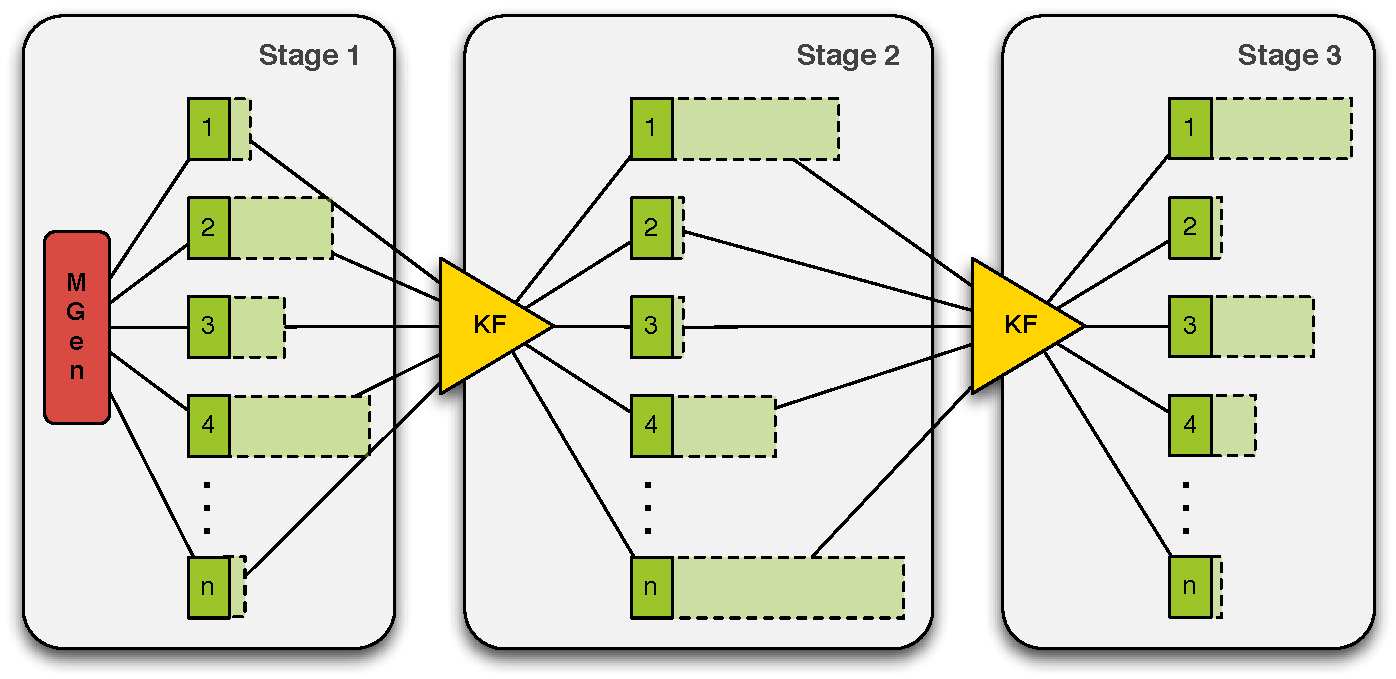
\includegraphics[scale=0.30]{./figures/3StageKalmanFilter}
\end{center}
\caption{ }
\label{fig:irregular_execution}
\end{figure}

\subsection{Application Outline}

The aim of our model application is to show the potential and ease of
use of a SAGA-enabled Cactus framework application. Our application
consists of a exemplary distributed simulation that uses the added
SAGA functionality to dynamically determine its ideal migration target
based on ad-hoc and statistical network characteristics and to migrate
itself in a heterogeneous Grid environment.  Although this a model
application it can be easily adapted to more complex scientific
applications.  Furthermore, our model application can be used as an
autonomous benchmarking agent for Grid resources. In this section we
briefly describe SAGA and the Cactus framework and discuss our
motivation to use SAGA to incorporate high-level Grid functionality
into Cactus.



\begin{figure}
\begin{center}
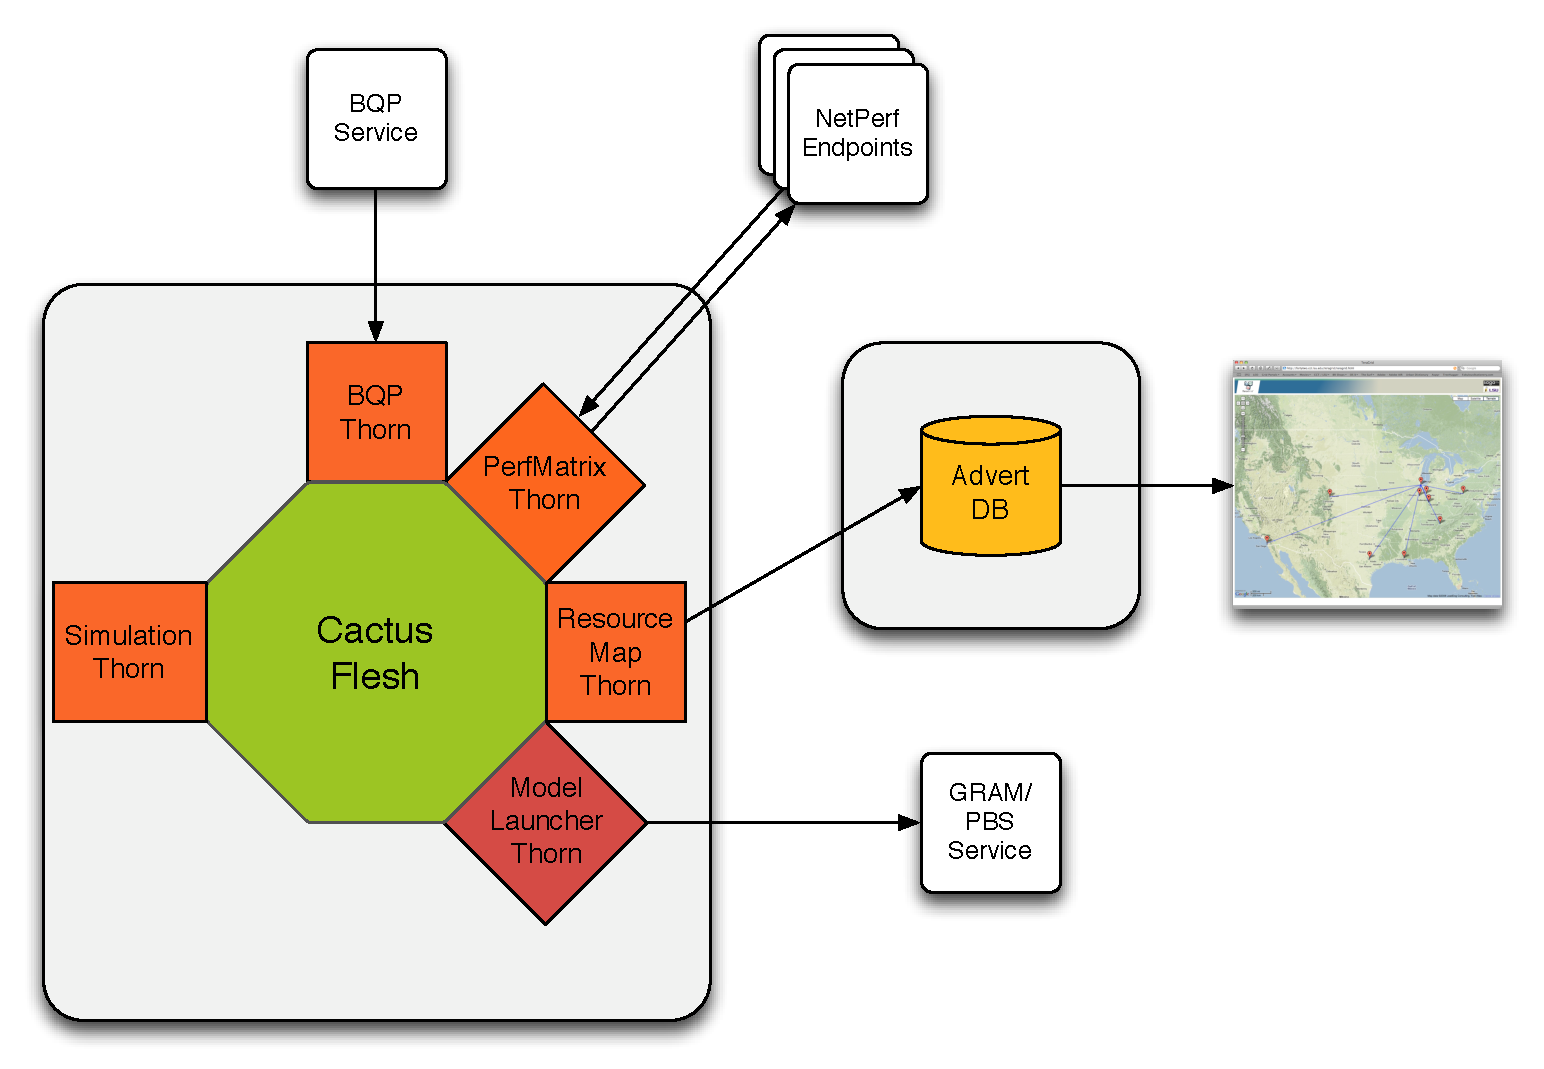
\includegraphics[scale=0.30]{./figures/ApplicationArchitecture}
\end{center}
\caption{}
\label{fig:application_architecture}
\end{figure}


\subsubsection{SAGA}

The Simple API for Grid Applications (SAGA) is an API standardization
effort within the Open Grid Forum (OGF)~\cite{ogf_web} -- an
international committee that coordinates the standardization of Grid
middleware and architectures.  The specification and implementations
of the SAGA API has been guided by detailed examination of the
requirements expressed by existing and emerging distributed computing
applications in order to find common themes and motifs that can be
reused across more than one use-case.  The main governing design
principle for the SAGA API is the 80:20 Rule: "Design an API with 20\%
complexity that serves 80\% of the application use cases".  They are
intended to cover the most common application-level distributed
computing programming constructs such as file transfer, and job
management.  In general, SAGA embodies the most commonly required
features derived from a broad survey of the community and provides the
most common grid programming abstractions that were identified by
several use cases.

SAGA provides a simple, POSIX-style API to the most common Grid
functions at a sufficiently high-level of abstraction so as to be able
to be independent of the diverse and dynamic Grid environments.  The
SAGA specification defines interfaces for the most common
Grid-programming functions grouped as a set of functional packages.
Version 1.0~\cite{saga-core} of the specification has been submitted
to the OGF editorial pipeline and is currently under review.  It
defines the following packages:

\begin{itemize}
\item File package - provides methods for accessing local and remote
  filesystems, browsing directories, moving, copying, and deleting
  files, setting access permissions, as well as zero-copy reading and
  writing
\item Replica package - provides methods for replica management such
  as browsing logical filesystems, moving, copying, deleting logical
  entries, adding and removing physical files from a logical file
  entry, and search logical files based on attribute sets.
\item Job package - provides methods for describing, submitting,
  monitoring, and controlling local and remote jobs. Many parts of
  this package were derived from the largely adopted
  DRMAA~\cite{drmaa_url} specification.
\item Stream package - provides methods for authenticated local and
  remote socket connections with hooks to support authorization and
  encryption schemes.
\item RPC package - is an implementation of the GGF GridRPC
  API~\cite{gridrpc_url} definition and provides methods for unified
  remote procedure calls.
\end{itemize}

The two critical aspects of SAGA are its {\it simplicity} of use and the
fact that it is well on the road to becoming a community {\it standard}.
It is important to note, that these two properties are 
provide the added value of using SAGA for Grid application development.
Simplicity arises from being able to limit the scope to only the most
common and important grid-functionality required by applications.
There a major advantages arising from its simplicity and imminent
standardization.  Standardization represents the fact that the
interface is derived from a wide-range of applications using a
collaborative approach and the output of which is endorsed by the
broader community.

The SAGA C++ reference implementation~\cite{saga_web} was incorporated
into the Cactus Code Framework in Ref~\cite{escience07} to provide the
needed Grid programming functionality. 

We believe this was an important step in merging two programming
abstractions to achieve an effect that is greater that sum of the
parts.

The SAGA C++ reference implementation is being developed in close
conjunction with the OGF standard.  Advert-service package which will
most-likely be incorporated into a future version of the OGF standard.
The SAGA C++ reference implementation comprise a complete set of local
adaptors, an SQlite3 and PostgreSQL advert-service adaptor, and Globus
pre-WS adaptors for file (GridFTP) and job (GRAM2) packages. We will
go onto show how the application uses these features.

\subsubsection{The Cactus Code~\cite{cactus_web}}

\CC{Need to reduce in length}

Cactus~\cite{X0} is a framework for high performance scientific
computing designed for scientists and engineers to develop and run
codes for solving complex problems.  Developing code for high
performance parallel machines has many challenges including
scalability, efficiency (for computation, communication and
input/output), portability and flexibility. Frameworks such as Cactus
allow scientists and engineers to develop modules which can then be
used together with modules written by other researchers to solve
complex computational problems. The framework provides tools ranging
from basic computational building blocks to complete toolkits that can
be used to solve complex problems in astrophysics, computational fluid
dynamics or other disciplines.  Tools developed in the Cactus Code
framework run on a wide range of architectures including desktop PC's,
supercomputers and computational Grids. Cactus and its associated
toolkits are publicly available for download from the Cactus Code
website.

From an architectural standpoint, the Cactus Code framework consists
of a central part (the ``flesh") and code modules (``thorns").  The
flesh serves as a module manager, scheduling the routines of the
thorns and passing data between thorns.  Thorns perform tasks ranging
from setting up the computational grid, decomposing the computational
grid for parallel processing, providing boundary and initial
conditions, communication of data from one processor to another,
solving partial differential equations to input and output and
visualization streaming. There are code modules that provide
simulation control tools, such as the HTTPD thorn that sets up a web
server for the simulation and allows researchers to control a
simulation or view sample output from a web interface.  Thorns can
also provide custom developed scientific or engineering applications,
such as computational fluid dynamics or gravitational physics.

Features of Cactus which make it particularly suited to take advantage
of a Grid environment include its portability, architecture
independent checkpoint and restart capabilities, steering interface,
and a well designed interface in the flesh for providing information
about grid variables, scheduling, parameters and so on.

Cactus has been a driving application for many Grid computing
projects.  An early experiment in 2000 called the Cactus
Worm~\cite{X1} showed how any Cactus application could be autonomously
migrated around the resources of the eGrid in Europe simply by adding
a new thorn which used the Globus MDS, GRAM and GridFTP APIs to access
Grid capabilities. A later collaboration with the GRADS project added
dynamic capabilities for resource selection and contract
negotiation~\cite{X2}.  These experiences led to the EU GridLab
project which experimented with Cactus migration as a driving
scenario~\cite{X3}.

Cactus was also used for early experiments in metacomputing, showing
how incorporating adaptive techniques into the Cactus driver layer,
such as dynamic load balancing, configuration of ghostzones, and use
of data compression could lead to acceptable scaling for large MPI
applications across multiple supercomputers. This work was awarded the
Gordon Bell prize in 2001~\cite{Cactus_GordonBell}.

\subsubsection{Why SAGA and Cactus?} 

Because of the modular structure of Cactus, any functionality provided
by a specific thorn is immediately available to any of the other
thorns in the configuration. For this reason we implemented a set of
new Cactus thorns providing an extensible set of functions allowing
the collection of netperf~\cite{netperf_web} based network performance
metrics. Additionally, the extensible nature of this set of thorns
permits additional metrics for any Cactus based application in the
future.  To integrate SAGA functionality into Cactus, a SAGA thorn was
developed that provides the basic SAGA installation information
(header files, libraries etc.)  to the thorns that require SAGA
capabilities.  SAGA provides different packages with a consistent and
uniform flavor, thus implementing thorns that have different
functionality (performance measurement and migrate thorns) using
different SAGA packages is preferable. Last but not least, using SAGA
and Cactus enables applications to specify and customize the network
performance characteristics that it needs; as we shall see later, the
ability to do so is a very useful feature.

\CC{need to add stuff about saga providing the ability to support
  programming models such as grid-superscalar and programming patterns
  such as task-farm and parameter sweeps; Ole a need to get a proper
  reference for this!}

\subsubsection{BQP}

Need a section on the basics theory and working of BQP

\subsection{Motivation: History Matching: Jha, Yaakoub} 

Modern reservoir simulators are in essence computer programs that are
used to model fluid flow in porous media. Reservoir flow modeling
exists in the context of of the resrvoir manamgenet function, a
process that optimizes the interaction between data and decision
making during the life cycle of a field.  One of the more popular
popular models is the Black Oil model that is used to solve for the
multi-component, multi-phase flow of oil, water and gas.  [ref Aziz,
Franchi].Typical input to a reservoir simulator consists of the
initial conditions of both fluids (saturation, temperature, pressure,
density etc...) as well as rock (porosity, permeability, depth etc...)
as well as the reservoir completion information (number of wells,
their location, their types: injectors or producers etc...).  This is
complicated by the fact that there are no accurate estimates of rock
properties or fluid saturations.

To ensure the fidelity of the reservoir model (or in most cases,
models) to the actual resrvoir, data from the reservoir model is
compared with production data. This process is referred to as
history matching. In this process, a large number of simulations of
the reservoir, each with different parameters or initial data, are
run and their results fitted against the production data. The
fitting method can be anything from a genetic algorithm, an ensemble
Kalman filter or a simulated annealing process. When model results
vary from production data, the model parameters are modified to bring
the model closer to the real production data. This process is repeated
until a good history match is produced. One of the best methods to perform
such history matching is the ensemble Kalman filter method, and it requires
a hard syncrhonization point where it gathers all the data from all the various
models and modifies model parameters to get better history matching in the
iterations to follow.

  When model results vary from production data, the model parameters
  are modified to bring the model closer to the real production data.
  This process is repeated until a good history match is produced. One
  of the best methods to perform such history matching is the ensemble
  Kalman filter method, and it requires a hard syncrhonization point
  where it gathers all the data from all the various models and
  modifies model parameters to get better history matching in the
  iterations to follow.

Typical reservoir simulations can vary in size from 100 grid points to
tens of millions of grid points, and a decent model space can contain
upwards of hundreds of models each with possibly varying size,
physical model (i.e equations to solve) and more importantly different
rock and fluid properties.  The variation in rock and fluid properties
has a direct and sizeable influence on the stiffness of the nonlinear
system of equations that needs to be solved, thus varying the required
runtime of different models.

Varying parameters sometimes also lead to varying systems of equations,
for example when the pressure in an oil reservoir becomes lower than
bubble-point pressure, which creates another phase, the vapor phase 
in the reservoir that needs to be solved. This obviously increases the size
requirement (by about one third). Another source of variation in size
is the fact that the stiffness of the matrix might become too large to solve
with the implicit-pressure explicit saturation formulation, and the model
would need a fully implicit formulation to converge. This effectively doubles
the number of the system of equations, and more than doubles the memory
required to solve the system of equations.

Hence a mechanism to assign models to available resources based on their
expected time to completion is useful. Such a mechanism would estimate the time
a model will spend in the queue of a resource, the time it needs to run, and the time
required to migrate the data it requires/produces back and forth, and based on that
attempt to minimize the time required to perform each history matching iteration.
In fact, with changing resource simulation requirements 
(as is the case with models that find themselves
lagging behind the rest of the model pack), a mechanism which can take
advantage of of faster, cheaper or more powerful machines is even more
advantegous \ref{reference first SAGA-Cactus paper}.

Hence a mechanism to automatically migrate a
simulation to another machine is useful. With changing resource
requirements during a simulation (as is the case with adaptive mesh
refinement) a mechanism which can take advantage of faster, cheaper or
more powerful machines is even more advantageous than simple
migration. As the primary Cactus simulation starts, it progresses
through the schedule of the routines in the configuration. One of
these routines regularly checks for the time left for the simulation
in the queue. Once that time is near a certain limit, usually a value
set by the user, a checkpoint of the simulation is forced and the
simulation termination routines are called. Checkpoint files can vary
in size from a few Gigabytes to a few TeraBytes and generally depend
on the size of the problem being solved. Blackhole Cactus simulations
run on up to thousands of processors and checkpoint to around 500
MegaBytes per processor ~\cite{Cactus_CCTTR} ~\cite{Cactus_Kamil06a}
~\cite{Cactus_Shalf05a}. With many terabytes of data that need to be
transferred, the knowledge of which resources can be readied first
will be important.

\subsection{Additional Use Cases}
We present three different usage scenarios; the first two represent
classes of application, while the third is related to the specific
case of remote visualization on optical lightpaths. We illustrate how
all three use cases can benefit greatly from our model applications or
minor variants thereof.

\subsection{Talk about additional 'irregular execution' applications}

% \subsubsection{Tightly-Coupled Applications}

% We pose the following questions: If a tightly-coupled application, say
% a distributed MPI code, had N potential resources to chose from, which
% M should it choose based upon network performance connecting those M
% resources?  As a distributed MPI applications, requires all-to-all
% communication, if we choose M out of N resources, then there are $N!
% \over M! (N-M)!$ possible combinations.  Which of these combinations
% will have the best network performance and thus how to choose the best
% M out of N resources~\cite{clade06}.  

% Given a fixed partition scheme, the general problem of how to
% distribute an application over M resources is a non-trivial one.
% There are potentially two distinct, orthogonal issues that need to be
% considered: choosing resources that provide optimal scheduling versus
% optimal distribution (network performance).  It is possible that the M
% resources to choose are not necessarily the optimal M to choose from a
% scheduling perspective, i.e., it is plausible that they have very
% different queue load factors, or one or more of the M resources have
% the longest wait times.  Resolving this coupled problem is not within
% scope of this paper - it requires extension to the information
% services that SAGA provides currently, so as to interact additionally
% with something like the Network Weather
% Service~\cite{wolski_cluster05, wolski_acm03, wolski_ccgrid02}.  But
% assuming that the M resources are computationally equal, the problem
% then becomes an issue of how to partition the problem such that
% communication is optimal.

Having determined which M resources to use, the way forward could be
using a Grid co-allocator such as HARC~\cite{harc_url}; that is,
having identified the best M resources from a network performance
perspective, we leave the co-scheduling of these M resources to HARC
which is an implementation of Paxos (two-phase) Commit Algorithm. We
will report on the interfacing of HARC with SAGA in the future.


\section{Application Implementation and Control Flow} 

\subsection { Application Architecture} 

\subsubsection{BQP Thorn?}
The BQP thorn is module in Cactus responsible for retrieving the BQP
information using the BQP api. The thorn iterates over all resources in a given
resource list, finds the resource and queue where if submitted, a reservoir
simulation (or model) of a given size and expected run time,
 will have a good chance (or high confidence) 
of getting through the queue and start running the earliest. Confidence
is in essence the probability that the job will run, and to obtain a confidence of
1.0, a high queue time is required. For history matching purposes, we found that
a confidence of 0.75 works well enough.

The information from the BQP thorn is retrieved for all reservoir simulations that 
need to be run, particularly the time in queue. The time in queue is added to the
time required to run the simulator (which is a function of the number of nodes
and resource used and is retrieved from regular application benchmarks) and the
time required to transfer data (that is obtained from the PerfMatrix thorn).
That time would be the estimated time to completion a given models in a given history matching
stage.

\subsection{ResourceMap Thorn}
The ResourceMap thorn maps the various models to available resources.
Each reservoir model has its own parameters that influence the size of
the model and the wall time it will need to finish. The ResourceMap
thorn queries the BQP thorn for the best machine and queue combination
that will start the model earliest at a high enough confidence (i.e
above a specified threshold). Once a machine/queue combination is
selected, the ResourceMap thorn calls functions in the Submit thorn to
submit the model.

\subsection{Submit Thorn}
The Submit thorn, as its name suggests, submits a job described by the ResourceMap
thorn to a given resource. A parameter file for the reservoir simulator and submission script are created at the resource using SAGA. A SAGA job is then launched that performs the actual submission (e.g qsub job\_1701.pbs).

\subsubsection{PerfMatrix} The PerfMatrix thorn takes care of the
intrinsic network performance measurement and persistent storage of
the results. Currently, the implementation uses
netperf~\cite{netperf_web} to measure unidirectional end-to-end
throughput. Netperf is implemented as a simple client-server model
consisting of two executables:
\begin{itemize}
\item{netserver: the measurement endpoint waiting for incoming connections}
\item{netperf: the initiator of a measurement connecting to a netserver endpoint}
\end{itemize}

The PerfMatrix algorithm uses a list of computational resources which
are potential migration targets for the application. After starting
up, the initial application spawns itself onto all available hosts.
\footnote{This approach is different from the original non-centralized
  spawning scheme shown in Fig.~\ref{fig:algo} The reason for our
  implementation using centralized spawning is the Globus Toolkit's
  (4.0.5) inability of full credential forwarding.} Once all jobs have
been launched, the original spawning application first establishes
netperf connections with all the spawned applications; this is
followed by the spawned applications establishing netperf connections
amongst each other, following the scheme shown in Fig.~\ref{fig:algo}.
The job spawning, control, and I/O redirection is done entirely using
SAGA's job management package.  Once a netperf process returns a
throughput result, the PerfMatrix thorn uses the SAGA advert-service
package to announce the result to a central PostgreSQL database which
is also used as a centralized logging facility. After all netperf
processes have finished and published their results, the database
contains a host-to-host throughput performance matrix along with a
timestamp which is available to other thorns as well as other
applications.

\subsubsection{Advert-service database} SAGA's advert-service package
describes a key-value based hierarchical attribute interface for
storing arbitrary information. The currently available adaptor is
capable to map these structures to an relational SQL schema and store
them in local (SQLite) and remote (PostgreSQL) RDBMS.

SAGA's advert-service offers a convenient way to simplify the
difficult task of centralized data collection and logging within
distributed applications. The advert structure consists of two
hierarchical trees: one for logging (containing the host name, a
timestamp, and the log message) and one for the throughput performance
matrix (containing a timestamp and the matrix itself). Since every
matrix is stored with a timestamp, every time the NetPerf thorn gets
triggered, an additional matrix is added to the advert-service which
leads to a growing stack of time-series data. This time-series can in
turn be analyzed by the SAGAMigrate thorn to determine if and where
to migrate.  Since all data stored in the advert-service can be
directly accessed using SAGA's high-level interface, it is easy to
browse the time-series data from other applications. A simple tool
that generates boxplots (Fig.~\ref{fig:boxplot}) from the performance
matrices is proof of the simplicity.

\subsubsection{SAGAMigrate} The SAGAMigrate thorn is a Cactus thorn
written in C++ that uses SAGA functions (for example file.copy and
job\_description.create\_job) to perform a simulation migration.
SAGAMigrate copies a restart parameter file and the checkpoint file(s)
from one machine to another (for example using the SAGA Globus
adaptors).

 \subsection{Control Flow} 

PerfMatrix measures the bandwidth between the primary simulation host
and a list of other candidate hosts. The results are stored in a
table accessible to other thorns in the configuration. The
SAGAMigrate thorn scans the table for the best candidate host to
migrate to. Once the best candidate host is selected, the SAGAMigrate
thorn copies the checkpoint and parameter files from the primary host
to the best candidate host and restarts the Cactus simulation to pick
up where it had left off on the primary host.

The current implementation has SAGAMigrate select the best host based
on the maximum bandwidth connectivity to that host. Our current
implementation uses SAGAMigrate parameters, variables that can be set
at runtime and are steerable, to set the network benchmark executable.
With steerable parameters, the user can decide at runtime what the
best metric is and set the appropriate benchmark parameters in
SAGAMigrate. With a more sophisticated performance metric the
selection algorithm would require revision beyond the current
``maximum bandwidth'' approach, for example measurements to be made,
by a query to the Network Weather Service ~\cite{NWS_web, bqp_url} or
a small application benchmark to estimate time to completion.

Another use of SAGAMigrate is to move simulation results from one
machine to another to run a different application. A typical scenario
would be a Cactus simulation migrating its results to another machine
and starting an analysis tool, a data mining tool or a visualization
application. With a fully parameterized interface to both application
and data, the current implementation of SAGAMigrate can perform basic
workflow staging across machines and applications.

\subsection{Interfacing with Google Maps}

\section{Infrastructure Used \& Deployment Details}

\subsection{Infrastructure}



\subsection{Deployment}

The deployment of applications across a pool of heterogeneous machines
belonging to different Grids and organizations can be a difficult
task. Different versions and availability of libraries and compilers
makes every single machine a unique environment. Although it is
technically possible to stage-in all required applications and
libraries and even to compile the application sources on the fly using
SAGA, we decided to deploy pre-build binaries on all machines since
this exercise is not part of this work's focus.

Since both, the Cactus framework and SAGA aim to be as
platform-independent as possible, the deployment process was rather
straightforward - the only noteworthy problems occurred during the
initial attempt to build SAGA on LONI's 64bit AIX 5L nodes. The
problems were mainly caused by the IBM's xlC++ compiler's inability to
handle C++ partial template instantiation, a broken AIX pthread
implementation and the absence of usable debugging tools. Although the
deployment process on AIX was very time consuming it eventually led to
a vastly improved SAGA build system and a more conservative use of C++
template mechanisms which ensures the support of other non-standard
compilers.

\section{Results and Discussion}

\begin{figure}
\begin{center}
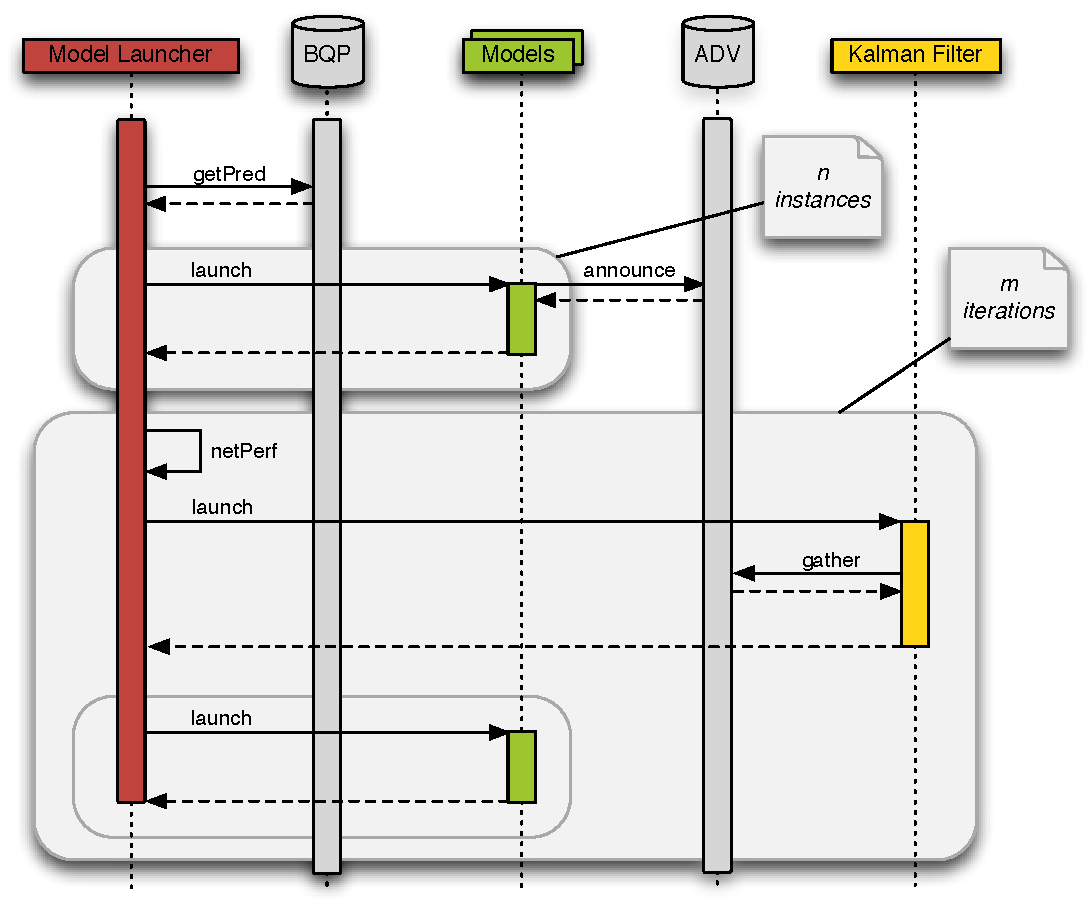
\includegraphics[scale=0.30]{./figures/SequenceDiagram}
\end{center}
\caption{ }
\label{fig:boxplot}
\end{figure}

\section{Future Work and Conclusion}

We will in future report on the performance of the execution of such
an application using a metascheduler such as Gridway.

\C{remove focus on adaptor development} Our experience should serve as
useful input to the community -- resource providers and middleware
developer - to support the development and deployment of SAGA
Adaptors.  We created a single set of Globus adaptors and deployed
them on distinct Grids. Our application successfully utilized these
adaptors, without any further customization, which goes to show that
the widespread availability of SAGA adaptors is an important step
towards the creation of distributed applications that can be
universally deployed (i.e.  independent of the details of the
resource's middleware and configuration detail).

We hope to motivate both middleware developers and resource providers
(such as TeraGrid, DEISA, EGEE, etc.) to subscribe to the SAGA
philosophy and thereby contribute to the development of SAGA adaptors
for their middleware stack as well as deploying these SAGA adaptors.

We also discussed how the deployment of this model application across
two distinct Grids was trivial as it only required the deployment of
of the appropriate SAGA adaptors.  Thus developing both applications
and tools using SAGA is an effective mechanism for ensuring
inter-operability across different middleware distributions -- even at
the application level -- something that is arguably missing in current
Grid Interoperation efforts~\cite{gin_paper}

Currently SAGA is in user space, but should ideally be supported at
the system level.

There are many applications that need to use federated
Grids~\cite{clade06, gin_paper}.  Utilizing SAGA to develop, or at
least provide Grid-functionality is a useful strategy. Therefore, if
the development and deployment of applications across federated grids
is to be facilitated, SAGA adaptor activity -- development and
deployment, needs to be self-sustaining and thus requires explicit
support, from both the middleware developers and resource providers.

The success of e-Science critically depends upon the availability of
e-Infrastructure.  But the promise of e-Science will be hollow without
delivery of the applications and application-enabling paradigms and
technology that can effectively utilize this new infrastructure. We
believe SAGA is an important first step in this direction.

\section{Acknowledgements}

This work has been made possible thanks to the internal resources of
the Center for Computation \& Technology (CCT) at Louisiana State
University.  Important funding for SAGA specification and development
has been provided by the UK EPSRC grant number GR/D0766171/1 (via
OMII).  We would like to acknowledge the support of the OGF SAGA
Research Group for their work towards developing the SAGA
specification, as well as the Cactus team. We would also like to thank
Carola Jesch for assistance with interfacing our output to google
maps. Additionally, we would like to acknowledge help from the LONI
support team and CyberInfrastructure Develompent group -- Prathyusha
Akunuri and Archit Kulshrestha.  Finally, we thank Rich Wolski (UCSB)
for unknowingly installing BQP on Queen Bee on time to make it usable
for this paper. Thanks Rich! Finally, SJ acknowledges the e-Science
Institute, Edinburgh for supporting the theme, ``Distributed
Programming Abstractions''.

\bibliographystyle{IEEEtran}
\bibliography{saga_clade08}
\end{document}

